 \documentclass{beamer}[10]

\usepackage{graphicx}
\usepackage{xcolor}
\usepackage{tabto}
%\usepackage{beamerthemesplit}
\usepackage{tikz}
\usepackage{cancel}
\usepackage{verbatim}
\usepackage{fancybox}
\usepackage{enumerate}
\usepackage{amsmath,amssymb,amsthm,textcomp,mathtools}
\usepackage[super]{nth}
\usepackage[amssymb]{SIunits}
\usepackage{booktabs}
\usepackage{cancel}
\usepackage{bm}
\usepackage[utf8]{inputenc}
\usepackage{tabularx}
\usepackage{ragged2e}
\newcolumntype{Y}{ >{\RaggedRight\arraybackslash}X}
\usetikzlibrary{arrows,shapes}
\newcommand\T{\rule{0pt}{2.6ex}}
\newcommand\B{\rule[-1.2ex]{0pt}{0pt}}
\definecolor{UUcrimson}{RGB}{204,0,0}
\mode<presentation>
{ \usetheme{default}
  \usecolortheme[named=UUcrimson]{structure}
  \useinnertheme{circles}
  \setbeamercovered{transparent}
  \setbeamertemplate{blocks}[rounded]
  \usefonttheme[onlymath]{serif}
  \setbeamertemplate{navigation symbols}{}
  \setbeamertemplate{footline}[page number]
  \setbeamertemplate{navigation symbols}{}
  \setbeamercolor{section in toc}{fg=black,bg=white}
  \setbeamercolor{alerted text}{fg=UUcrimson!80!gray}
  \setbeamercolor*{palette primary}{fg=white,bg=UUcrimson}
  \setbeamercolor*{palette secondary}{fg=UUcrimson!70!black,bg=gray!15!white}
  \setbeamercolor*{palette tertiary}{bg=UUcrimson!80!black,fg=gray!10!white}
  \setbeamercolor*{palette quaternary}{fg=UUcrimson,bg=gray!5!white}
  \setbeamercolor*{palette sidebar primary}{fg=UUcrimson!10!black}
  \setbeamercolor*{palette sidebar secondary}{fg=white}
  \setbeamercolor*{palette sidebar tertiary}{fg=UUcrimson!50!black}
  \setbeamercolor*{palette sidebar quaternary}{fg=gray!10!white}
  \setbeamercolor{titlelike}{parent=palette primary,fg=white}
  \setbeamercolor{frametitle}{bg=UUcrimson}
  \setbeamercolor{frametitle right}{bg=UUcrimson}
  \setbeamercolor*{separation line}{}
  \setbeamercolor*{fine separation line}{}
}

\usetikzlibrary{backgrounds}
\makeatletter
\tikzstyle{every picture}+=[remember picture]
\tikzset{%
  fancy quotes/.style={
    text width=\fq@width pt,
    align=justify,
    inner sep=1em,
    anchor=north west,
    minimum width=\linewidth,
    font=\itshape
  },
  fancy quotes width/.initial={.8\linewidth},
  fancy quotes marks/.style={
    scale=8,
    text=white,
    inner sep=0pt,
  },
  fancy quotes opening/.style={
    fancy quotes marks,
  },
  fancy quotes closing/.style={
    fancy quotes marks,
  },
  fancy quotes background/.style={
    show background rectangle,
    inner frame xsep=0pt,
    background rectangle/.style={
      fill=gray!25,
      rounded corners,
    },
  }
}
\newenvironment{fancyquotes}[1][]{%
\noindent
\tikzpicture[fancy quotes background]
\node[fancy quotes opening,anchor=north west] (fq@ul) at (0,0) {``};
\tikz@scan@one@point\pgfutil@firstofone(fq@ul.east)
\pgfmathsetmacro{\fq@width}{\linewidth - 2*\pgf@x}
\node[fancy quotes,#1] (fq@txt) at (fq@ul.north west) \bgroup}
{\egroup;
\node[overlay,fancy quotes closing,anchor=east] at (fq@txt.south east) {''};
\endtikzpicture}
\makeatother

\usepackage{scalerel}[2014/03/10]
\usepackage{stackengine}
\usepackage{empheq}
\newcommand*\widefbox[1]{\fbox{\hspace{0.5em}#1\hspace{0.5em}}}

\newcommand\reallywidetilde[1]{\ThisStyle{%
  \setbox0=\hbox{$\SavedStyle#1$}%
  \stackengine{-.1\LMpt}{$\SavedStyle#1$}{%
    \stretchto{\scaleto{\SavedStyle\mkern.2mu\sim}{.5467\wd0}}{.4\ht0}%
%    .2mu is the kern imbalance when clipping white space
%    .5467++++ is \ht/[kerned \wd] aspect ratio for \sim glyph
  }{O}{c}{F}{T}{S}%
}}
\usepackage{media9}

\logo{
\includegraphics[width=0.75cm]{logo.jpg}}
\author[Gibbs]{Dr. Jeremy A. Gibbs}
\institute{Department of Mechanical Engineering\\University of Utah}
\date{Fall 2016}
\title{LES of Turbulent Flows: Lecture 19}
\begin{document}

%----------------------------------------------------------------------------------------
%	TITLE & TOC SLIDES
%----------------------------------------------------------------------------------------

\begin{frame} 
  \titlepage
\end{frame}

%------------------------------------------------

\begin{frame}
\frametitle{Overview}
\tableofcontents
\end{frame}

%------------------------------------------------
\section{Statistical Conditions for a SGS Model} %
%------------------------------------------------
\begin{frame}{Statistical Conditions for a SGS Model}
\textit{a posteriori}
\begin{itemize}
	\item Project \#1 is based on \textit{a posteriori} model testing -- one particular way to test for a model's correctness
	\item The idea there is to use the model in a simulation and compare the output data with experimental data
	\item A downside to this testing approach is that it is hard to understand what physics are important for a model to work (or to fail)
	\item Another downside is the difficulty in separating the model from other influences, such as model numerics
\end{itemize}
\end{frame}
%------------------------------------------------
\begin{frame}{Statistical Conditions for a SGS Model}
\textit{a priori}
\begin{itemize}
	\item Project \#2 will be based on \textit{a priori} model testing -- a way to test for a model's physical robustness
	\item The idea there is to use some fully-resolved ``truth'' dataset (DNS, experiments) and filter them to some chosen scale
	\item The filtered data is used to compute the actual and modeled stresses, which are then compared
\end{itemize}
\end{frame}
%------------------------------------------------
\begin{frame}{Statistical Conditions for a SGS Model}
\textit{a priori}
\begin{itemize}
	\item A downside to \textit{a priori} model testing is that instantaneous comparison between real and modeled stresses often show poor correlation
	\item However, this does not necessarily translate into a ``bad'' result when performing \textit{a posteriori} tests
	\item In other words, \textit{a priori} tests can present an overly negative outlook for a model
	\item Thus, the use of both testing procedures is often required to make a fully-formed assessment of a model
\end{itemize}
\end{frame}
%------------------------------------------------
\begin{frame}{Statistical Conditions for a SGS Model}
What do we mean? See this from Stoll and Port\'{e}-Agel (2009)
\begin{figure}
	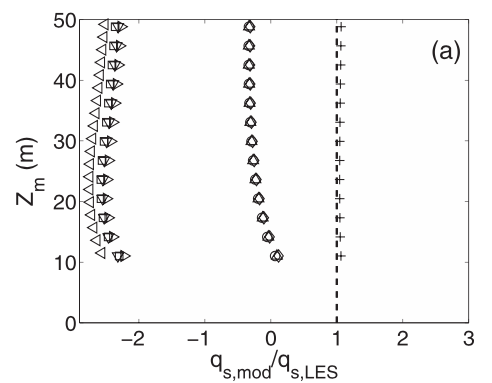
\includegraphics[width=0.6\textwidth]{apriori1}	
\end{figure}
Offline testing of schemes led to wrong sign of surface flux! But when coupled in a system, it can produce reasonable results.
\end{frame}
%------------------------------------------------
\begin{frame}{Statistical Conditions for a SGS Model}
\begin{itemize}
	\item Can we get around these issues related to \textit{a priori} tests?
	\item Yes! We can apply weaker conditions on our model that are ususal expected for \textit{a priori} tests
	\item The truth is that for many applications we simply do not care about a single realization of an LES
	\item Why? Well, we expect the flow to evolve chaotically -- so to expect perfect instantaneous relationships is not realistic
	\item Rather, we really care about whether the LES produces correct statistical features of a flow
\end{itemize}
\end{frame}
%------------------------------------------------
\begin{frame}{Statistical Conditions for a SGS Model}
\begin{itemize}
	\item Switching to a statistical \textit{a priori} framework leads to an obvious question - \textbf{what conditions should a SGS model satisfy?}
	\item Specifically we are interested in answering the question what statistical properties should $\tau_{ij}$ and $\tau_{ij}^{M}$ share?
	\item In other words, what specific properties must the model satisfy such that the real and LES low-order velocity statistics match in a reasonable way?  
\end{itemize}
\end{frame}
%------------------------------------------------
\begin{frame}{Statistical Conditions for a SGS Model}
We know a ``good'' model should adhere to our equations of motion
\begin{itemize}
	\item Invariance to translation, rotation, and reflection (in the absence of boundaries)
	\item Hopefully, invariance to Re
	\item Ideally, invariant to $\Delta$
\end{itemize}
~\newline
To get more specific than this, we need to talk about \textbf{statistics of SGS models} (Meneveau 1994)\\~\\
We want to know what properties $\tau_{ij}$ and $\tau_{ij}^{M}$ should share to produce reasonably accurate ensemble statistics of the velocity field
\end{frame}
%------------------------------------------------
\begin{frame}{Statistical Conditions for a SGS Model}
\begin{itemize}
	\item \textbf{To obtain correct \nth{1}- and \nth{2}-order moments} of our resolved field, our \textbf{model must} at least be able to \textbf{produce average modeled stresses} that match the ``real'' stresses
	\item This \textbf{doesn't guarantee that our \nth{2}-order moments are correct} -- it is only a necessary condition everywhere
\end{itemize}
\end{frame}
%------------------------------------------------
\begin{frame}{Statistical Conditions for a SGS Model}
\begin{itemize}
	\item \textbf{To produce \nth{2}-order moments}, we need to have our model reproduce \nth{2}- and \nth{3}-order SGS stats including stresses and correlations (\textit{e.g.} stress with velocity or stress with rate-of-strain tensor) that match the ``real'' values-- This includes \textbf{matching} $\mathbf{\langle \Pi \rangle}$ \textbf{everywhere} (recall that $\Pi$ is the SFS dissipation rate)
	\item For even higher order moments we need to match higher order SGS stats
\end{itemize}
\end{frame}

%------------------------------------------------
\section{Computing SGS Quantities}
%------------------------------------------------
\begin{frame}{Computing SGS Quantities}
\begin{itemize}
	\item Procedurally, \textbf{how do we compute these SGS stats from data} (DNS or experiments)?
	\item  Select your data (after quality control) and identify missing velocity or gradient terms
	\item Separate the data into resolved and SGS scales by calculating $\tilde{u}_i$ and $\widetilde{u_iu_j}$ with an appropriate LES filter (see lecture 5 for the most common examples)
\end{itemize}
\end{frame}
%------------------------------------------------
\begin{frame}{Computing SGS Quantities}
\begin{itemize}
	\item At this point, a decision must be made: \textbf{to down-sample or not} (see Liu et al. 1994)
	\item Down-sampling means removing points from the field that are separated (spatially) by less than our filter scale $\Delta$ (denoted by the $\sim$)
	\item Effectively this means we keep less points than we started with (e.g. from $128^3$ to $32^3$) after filtering
\end{itemize}
\end{frame}
%------------------------------------------------
\begin{frame}{Computing SGS Quantities}
Figure 6 from Liu et al. (1994)
\begin{figure}
	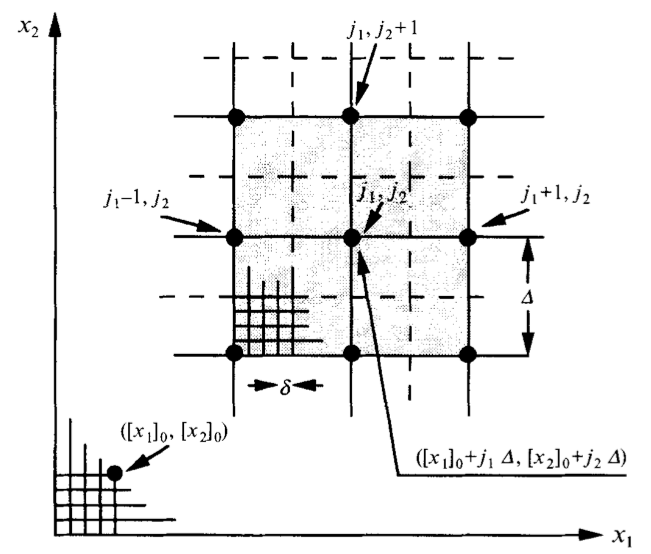
\includegraphics[width=0.8\textwidth]{apriori2}	
\end{figure}
\end{frame}
%------------------------------------------------
\begin{frame}{Computing SGS Quantities}
Downsampling
\begin{itemize}
	\item \textbf{Pros}: we get a ``true'' representation of the effect of gradient estimates on our SGS models and avoid enhanced correlations due to filter overlap
	\item \textbf{Cons}: we lose data points (important if we have limited data) and we now need to consider the above gradient estimation errors!
\end{itemize}
\end{frame}
%------------------------------------------------
\begin{frame}{Computing SGS Quantities}
\begin{itemize}
	\item  Calculate \textbf{local values} of all the components of 
	$$\tau_{ij}^{\Delta} = \widetilde{u_iu_j} - \widetilde{u}_i\widetilde{u}_j$$
	and
	$$S_{ij} = \left( \frac{\partial \widetilde{u}_i}{\partial x_j} + \frac{\partial \widetilde{u}_j}{\partial x_i}\right)$$
	\item You may need approximations here based on your data!
	\item  For some models you may need to calculate other parameters (\textit{e.g.}, mixed and nonlinear models) but the general procedure is the same
\end{itemize}
\end{frame}
%------------------------------------------------
\begin{frame}{Computing SGS Quantities}
\begin{itemize}
	\item Homework \#2 implemented different types of filters
	\item Once you have these basic quantities calculated you can calculate model values of $\tau_{ij}^{\Delta,M}$ and statistics of the actual (from data) and modeled SGS stresses including average values, correlation coefficients, and variances
	\item We can also calculate other SGS statistics like $\langle \Pi^{\Delta}\rangle = - \langle\tau_{ij}^{\Delta}\widetilde{S}_{ij}\rangle$ and $\langle \Pi^{\Delta,M}\rangle$ -- or any model coefficients of interest
	\item The following pages give some examples of SGS statistics and model coefficients calculated from various references
\end{itemize}
\end{frame}
%------------------------------------------------
\begin{frame}{SGS Dissipation $\Pi = -\tau_{ij}\widetilde{S}_{ij}$}
$\Pi$ from experiments in the Utah desert (Carper \& Port\'{e}-Agel 2004)
    \begin{columns}
    \begin{column}{.4\textwidth}
    \begin{minipage}[c][.6\textheight][c]{\linewidth}
    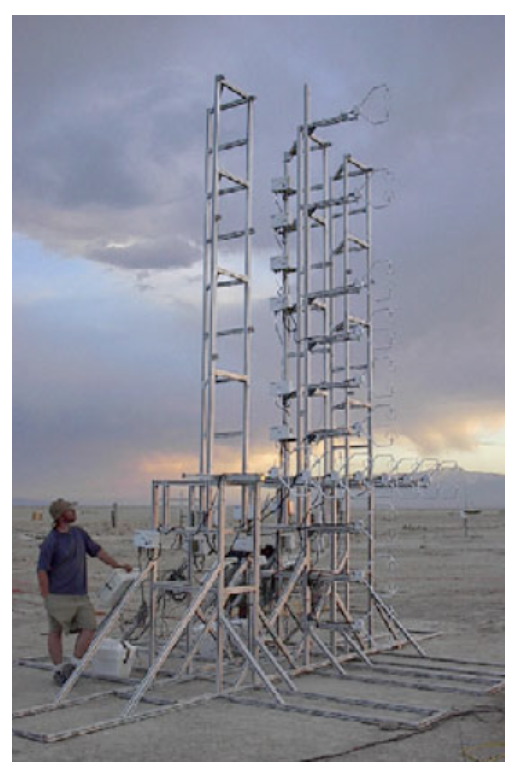
\includegraphics[width=\textwidth]{apriori5}
    ~\\\tiny{Experimental setup}
      \end{minipage}
    \end{column}
    \begin{column}{.6\textwidth}
      \begin{figure}
      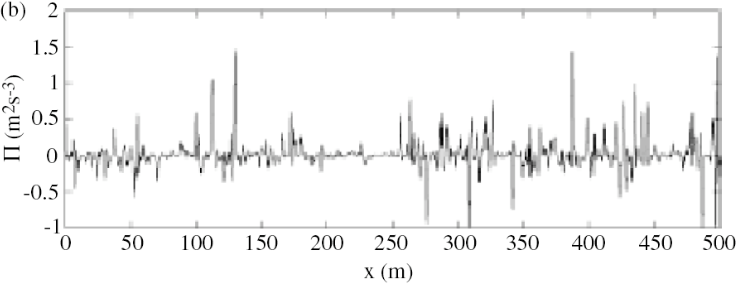
\includegraphics[width=0.9\textwidth]{apriori3}
      ~\\\tiny{Example time series of $\Pi$ from the ABL (late afternoon)}
      ~\\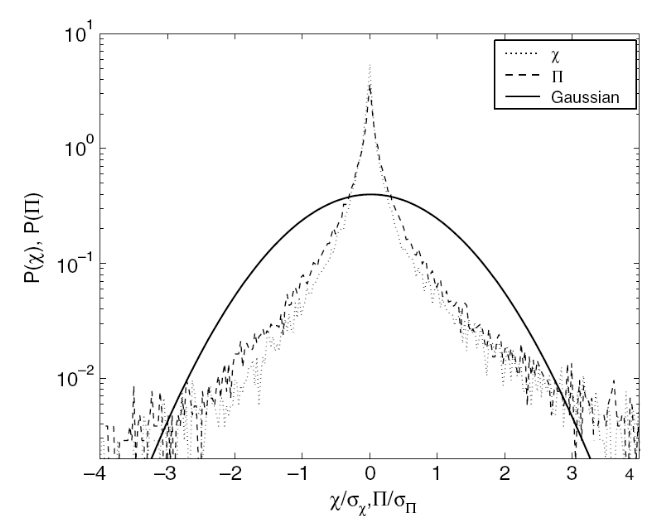
\includegraphics[width=0.7\textwidth]{apriori4}
      ~\\\tiny{Example PDF of $\Pi$ from the ABL (late afternoon)}
      \end{figure}
    \end{column}
  \end{columns}
\end{frame}
%------------------------------------------------
\begin{frame}{SGS Dissipation $\Pi = -\tau_{ij}\widetilde{S}_{ij}$}
$\Pi$ from wind tunnel experiments in a round jet (Liu et al. 1994)    \begin{columns}
    \begin{column}{.5\textwidth}
    \begin{minipage}[c][.8\textheight][c]{\linewidth}
    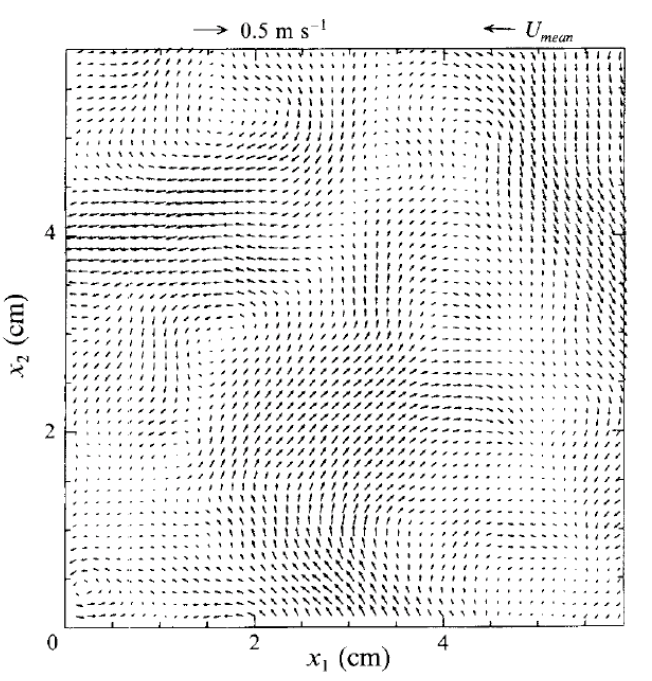
\includegraphics[width=\textwidth]{apriori6}
    ~\\\tiny{Top-hat filtered PIV field}
      \end{minipage}
    \end{column}
    \begin{column}{.5\textwidth}
      \begin{figure}
      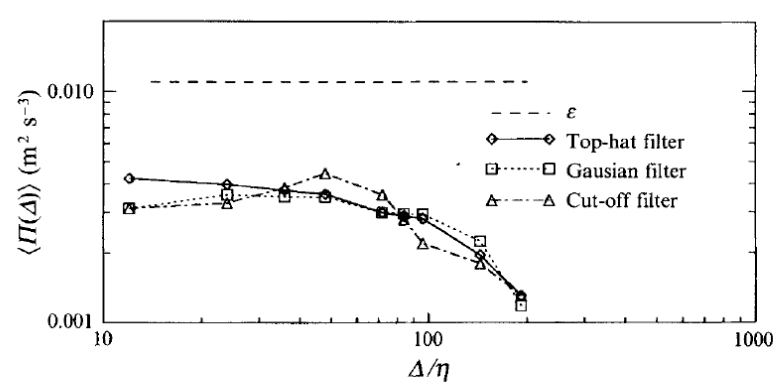
\includegraphics[width=0.9\textwidth]{apriori7}
      ~\\\tiny{Average $\Pi$ from the wind tunnel experiment compared to molecular dissipation}
      ~\\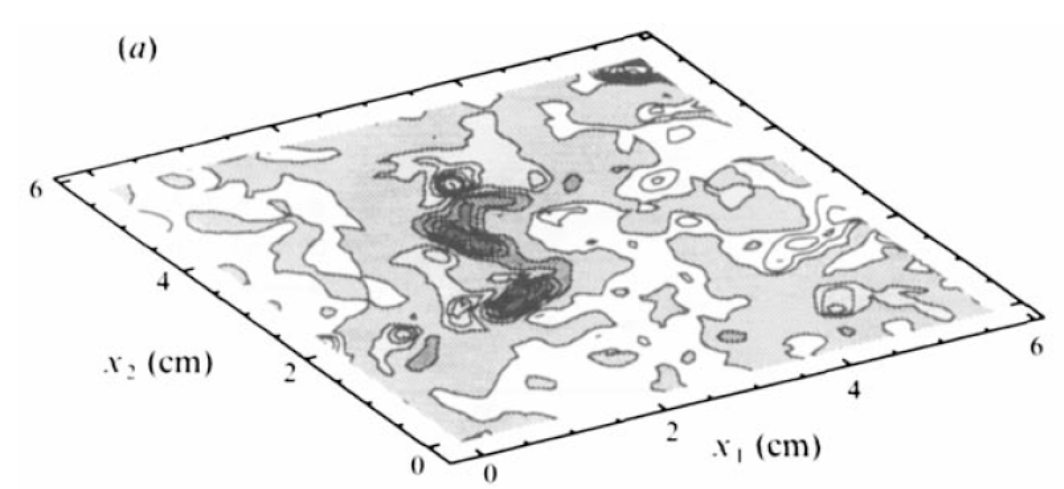
\includegraphics[width=0.9\textwidth]{apriori8}
      ~\\\tiny{Spatial distribution of $\Pi$ from PIV}
      \end{figure}
    \end{column}
  \end{columns}
\end{frame}
%------------------------------------------------
\begin{frame}{SGS Dissipation $\Pi = -\tau_{ij}\widetilde{S}_{ij}$}
$\Pi$ DNS of turbulent channel flow Re=3300 ($U_c$) (Piomelli et al. 1991)    \begin{columns}
    \begin{column}{.5\textwidth}
    \begin{minipage}[c][.4\textheight][c]{\linewidth}
    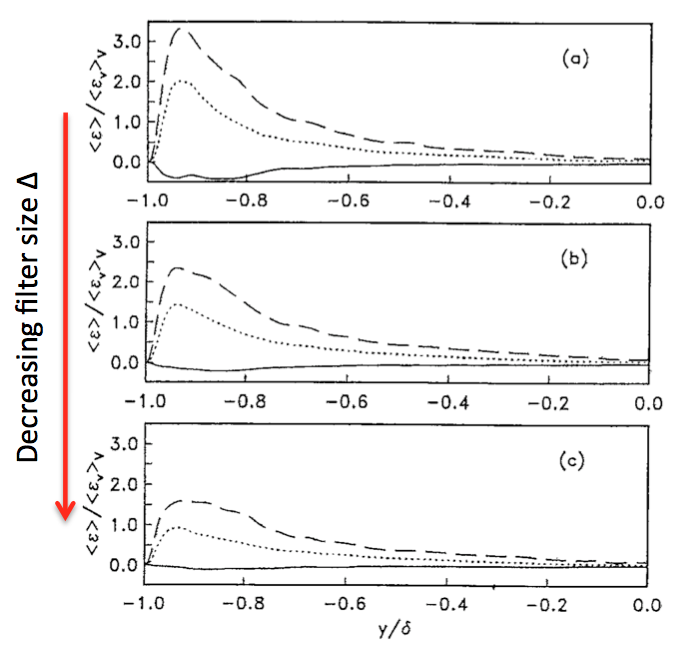
\includegraphics[width=\textwidth]{apriori9}
    ~\\\tiny{$\Pi$ normalized by the total dissipation \newline$-$ average; $--$ rms and $\cdot\cdot\cdot$ backscatter}
      \end{minipage}
    \end{column}
    \begin{column}{.48\textwidth}
      \begin{figure}
      ~\\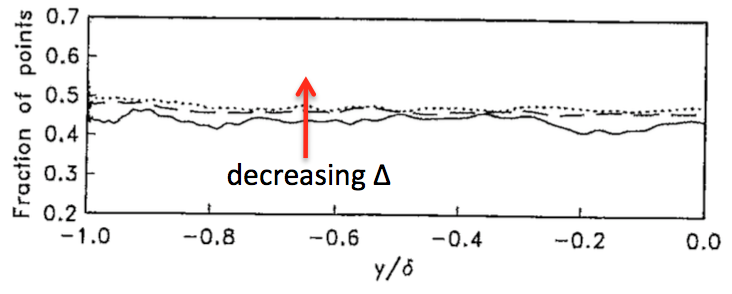
\includegraphics[width=1\textwidth]{apriori10}
      ~\\\tiny{Fraction of points in channel flow with backscatter for 3 different filter widths}
      \end{figure}
      \begin{itemize}
     	\small
      	\item backscatter increases with Re
      	\item fraction of backscatter points decrease for a Gaussian filter (cutoff results shown) to about 30\%.
      \end{itemize}
    \end{column}
  \end{columns}
\end{frame}
%------------------------------------------------
\begin{frame}{SGS SGS Model Correlation Coefficients}
Correlation coefficients from Clark et al (1979) for different models    \begin{figure}
	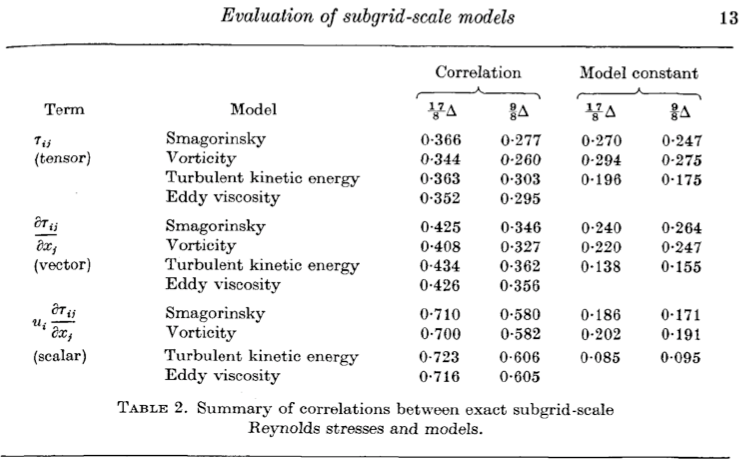
\includegraphics[width=0.8\textwidth]{apriori13}
\end{figure}
\vspace{-10pt}
\begin{itemize}
\small
	\item Eddy-viscosity - $\tau_{ij} = -2\nu_T \widetilde{S}_{ij}$
	\item Smagorinsky - $\nu_T = (C_s \Delta)^2 |\widetilde{S}_{ij}|$
	\item Deardorff - $\nu_T = (C_1 \Delta)^2 \widetilde{k}_{r}^{1/2}$
	\item Vorticity - $\nu_T = (C\Delta)^2(\omega_i\omega_i)^{1/2}$
\end{itemize}
\end{frame}
%------------------------------------------------
\begin{frame}{SGS SGS Model Correlation Coefficients}
Correlation coefficients from Clark et al (1979) for different models    \begin{figure}
	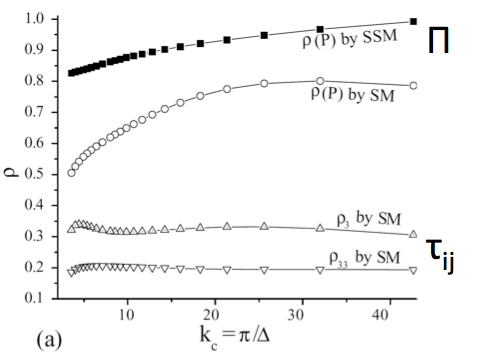
\includegraphics[width=0.4\textwidth]{apriori12}~\\\tiny{Correlation coefficients from Lu et al (2007) for Smagorinsky and Similarity models}
	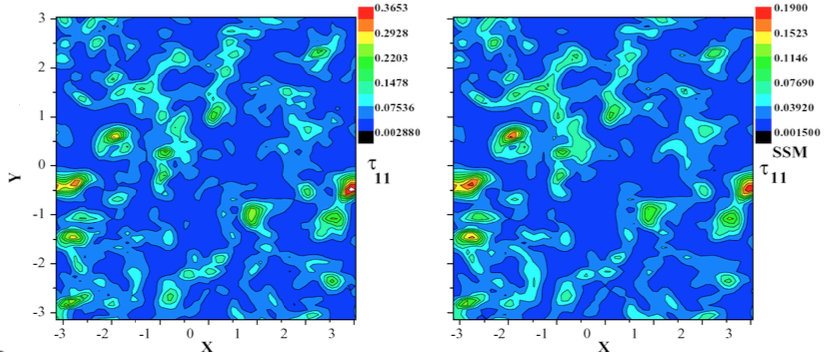
\includegraphics[width=0.75\textwidth]{apriori11}
	~\\\tiny{Measured (left) and modeled (right) with the similarity model $\tau_{11}$ from Lu et al (2007)}
\end{figure}
\end{frame}
%------------------------------------------------
\begin{frame}{SGS SGS Model Coefficient Estimation}
Model coefficients evaluated by matching $\Pi$ from ABL study of Sullivan et al (2003)    
	\begin{columns}
    \begin{column}{.4\textwidth}
    \begin{minipage}[c][.1\textheight][c]{\linewidth}
    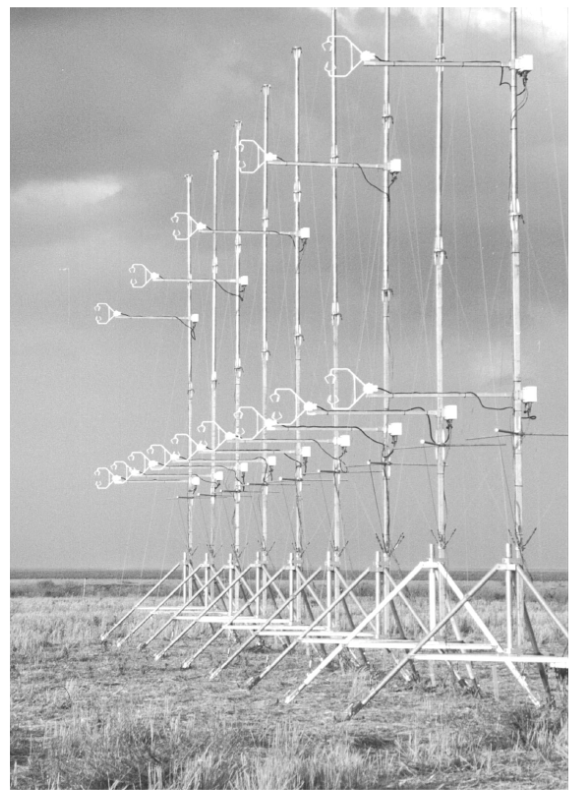
\includegraphics[width=\textwidth]{apriori14}
    ~\\\tiny{Experimental setup in Colorado}
      \end{minipage}
    \end{column}
    \begin{column}{.6\textwidth}
    \vspace{-10pt}
      \begin{figure}
      ~\\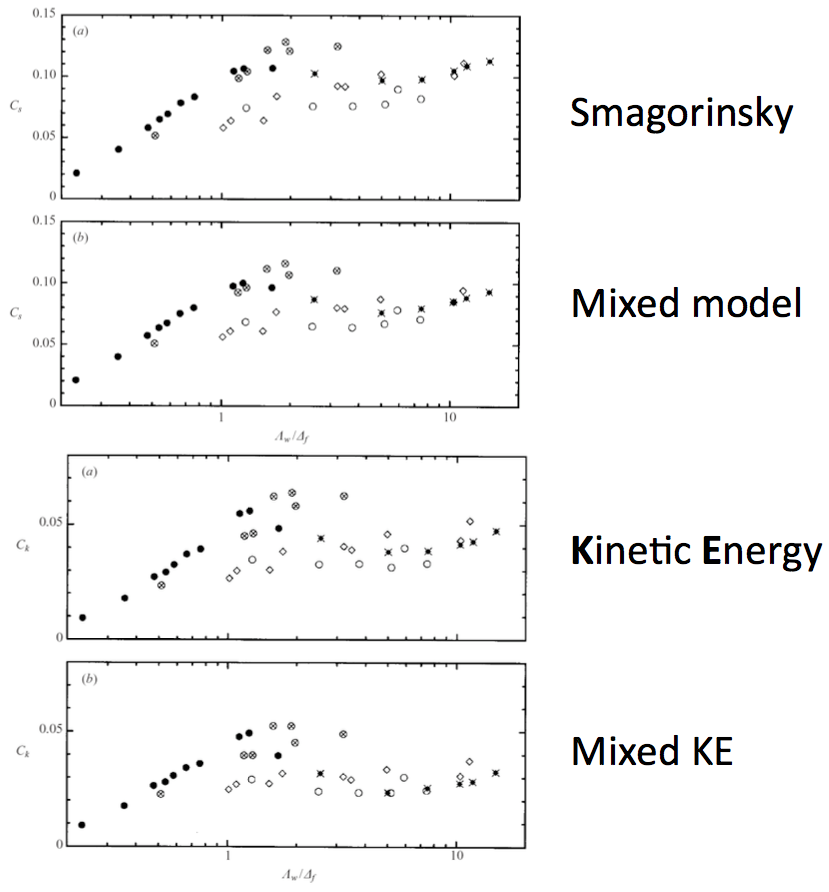
\includegraphics[width=0.95\textwidth]{apriori15}
      \end{figure}
    \end{column}
  \end{columns}
\end{frame}
%------------------------------------------------
\begin{frame}{SGS SGS Model Coefficient Estimation}
Smagorinsky coefficients with stability (Kleissl et al 2004) 
	\begin{columns}
    \begin{column}{.45\textwidth}
    \begin{minipage}[c][.9\textheight][c]{\linewidth}
    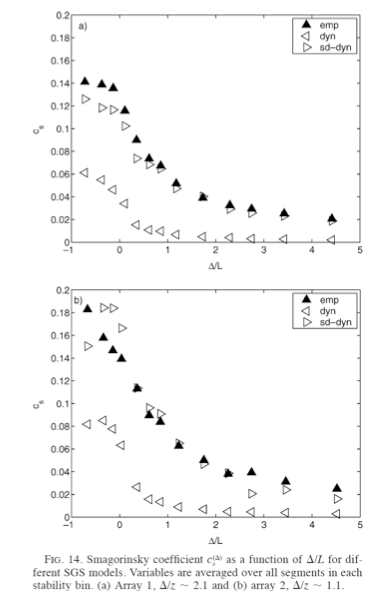
\includegraphics[width=\textwidth]{apriori16}
      \end{minipage}
    \end{column}
    \begin{column}{.6\textwidth}
    \vspace{-10pt}
      \begin{figure}
      ~\\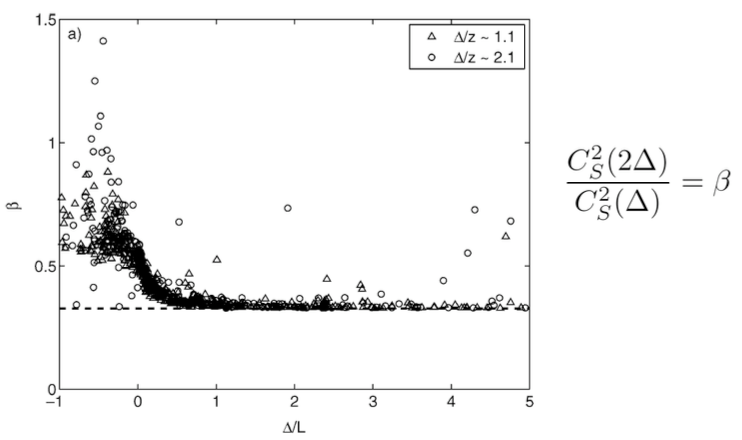
\includegraphics[width=1\textwidth]{apriori17}
      \end{figure}
    \end{column}
  \end{columns}
\end{frame}

%------------------------------------------------
\begin{frame}{SGS SGS Model Coefficient Estimation}
Smagorinsky coefficients with stability (Bou-Zeid et al. 2010)
$q_i^{\text{model}} = -k_{\text{SGS}}\partial \tilde{\theta}/\partial x_i = -\text{Pr}^{-1}_{\text{SGS}}(C_S \Delta)^2|\tilde{S}|\partial \tilde{\theta}/\partial x_i$
	\begin{figure}
		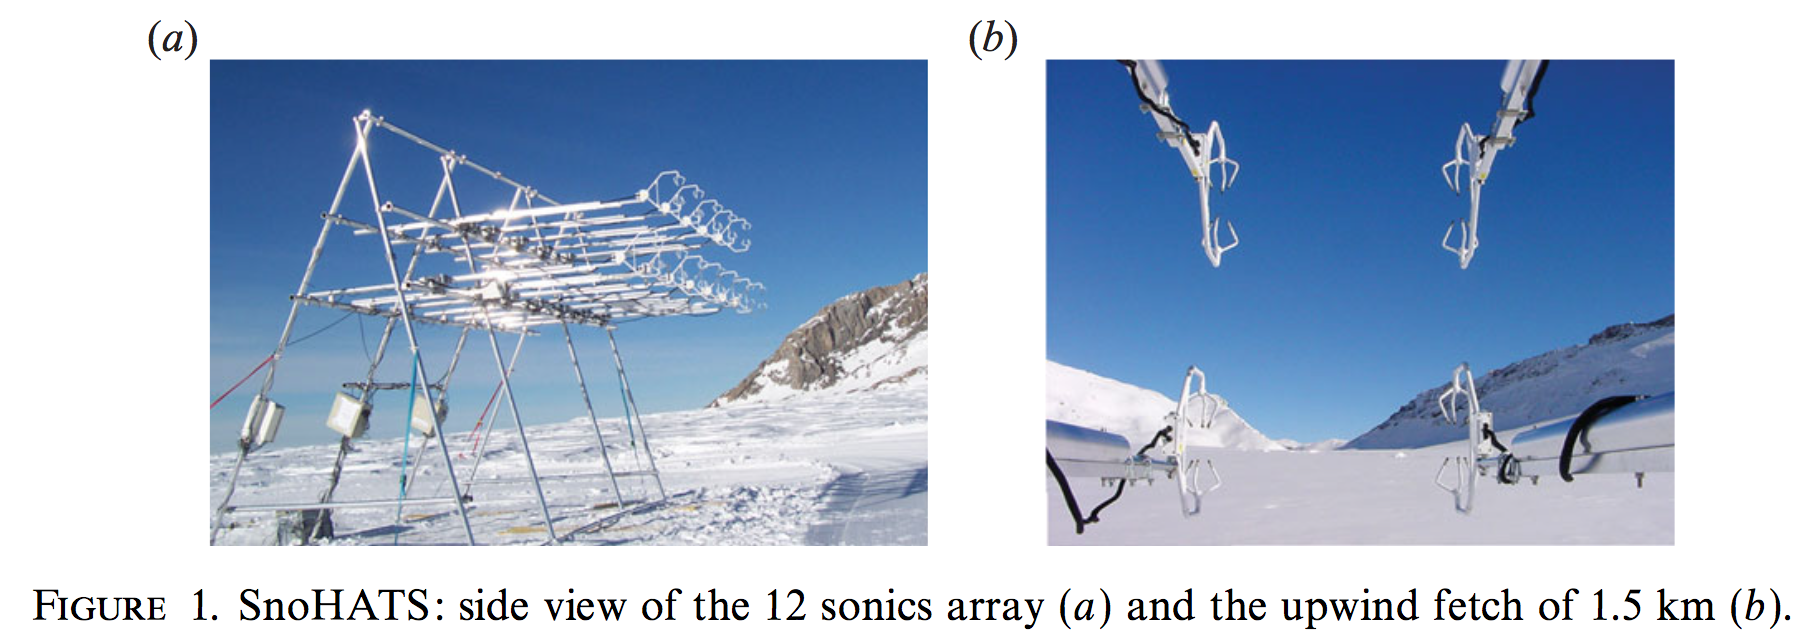
\includegraphics[width=0.7\textwidth]{apriori18}\\
		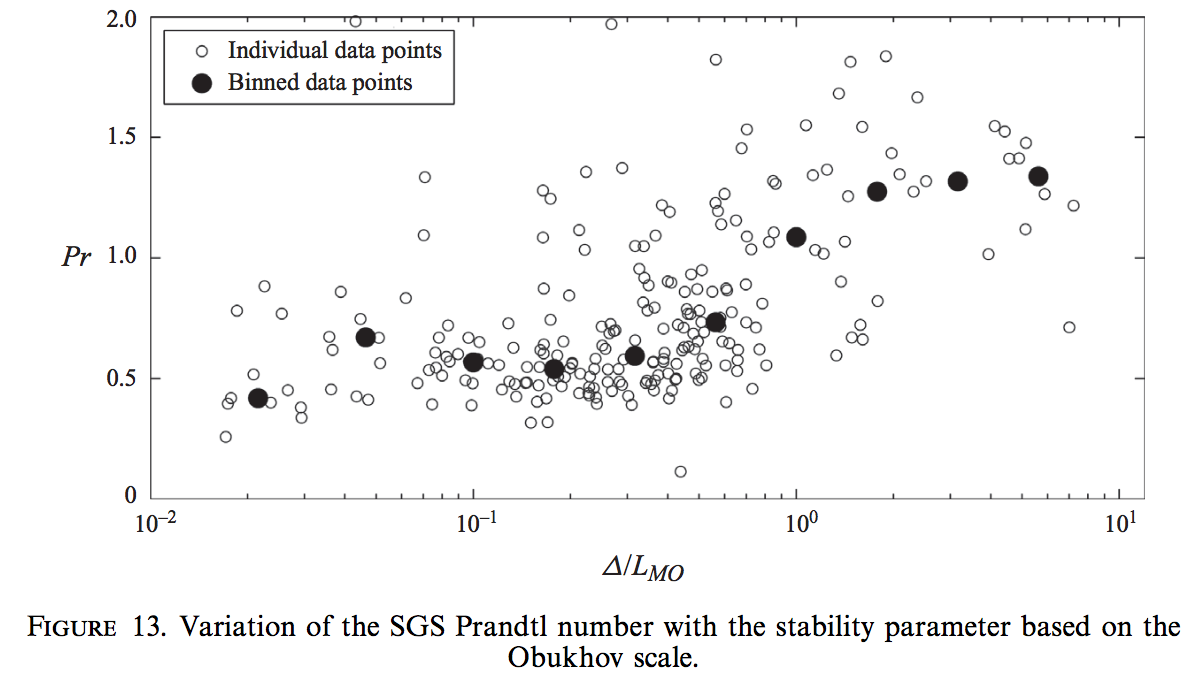
\includegraphics[width=0.7\textwidth]{apriori19}
	\end{figure}
\end{frame}

%------------------------------------------------
\begin{frame}{SGS SGS Model Coefficient Estimation}
Smagorinsky coefficients with stability (Bou-Zeid et al. 2010)
$q_i^{\text{model}} = -k_{\text{SGS}}\partial \tilde{\theta}/\partial x_i = -\text{Pr}^{-1}_{\text{SGS}}(C_S \Delta)^2|\tilde{S}|\partial \tilde{\theta}/\partial x_i$ 
	\begin{figure}
		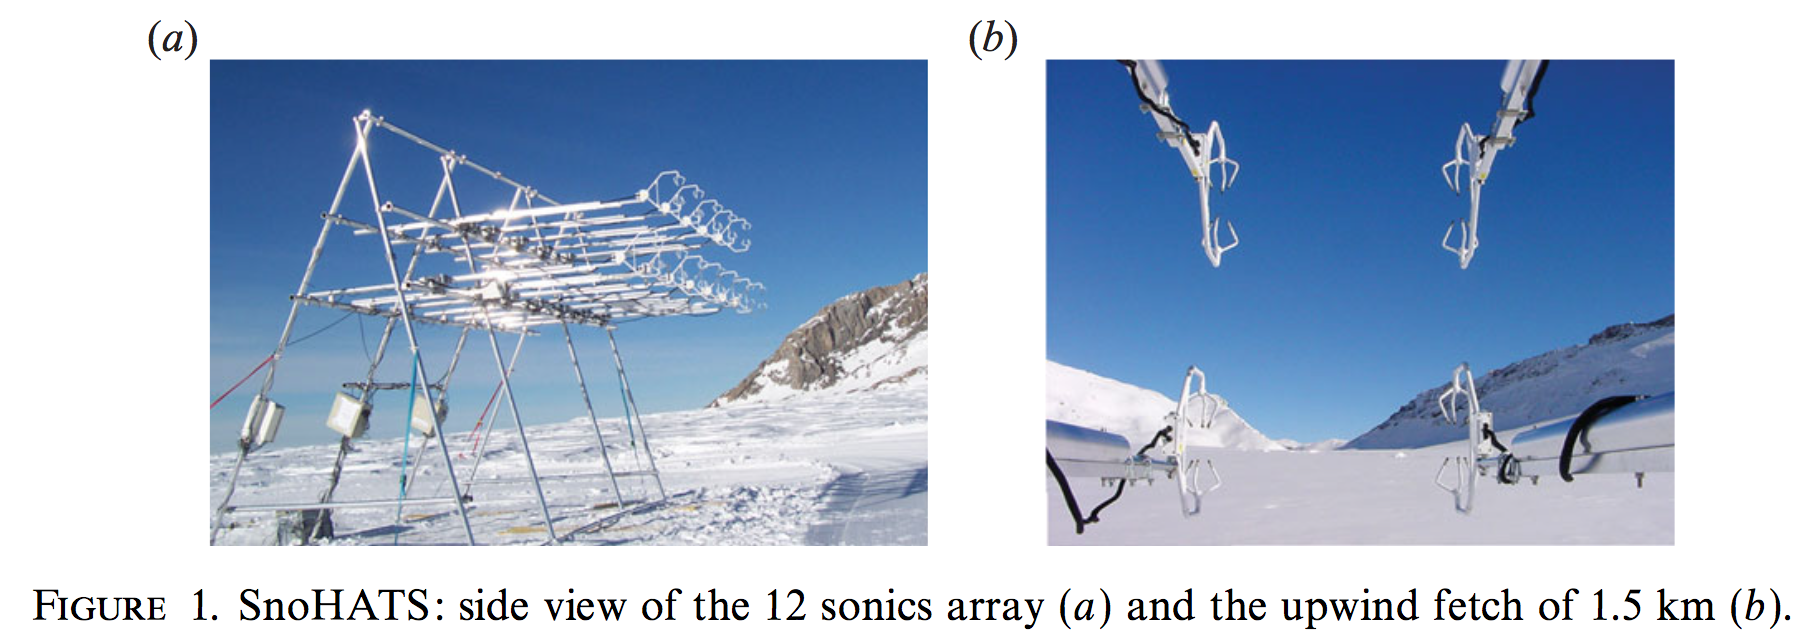
\includegraphics[width=0.7\textwidth]{apriori18}\\
		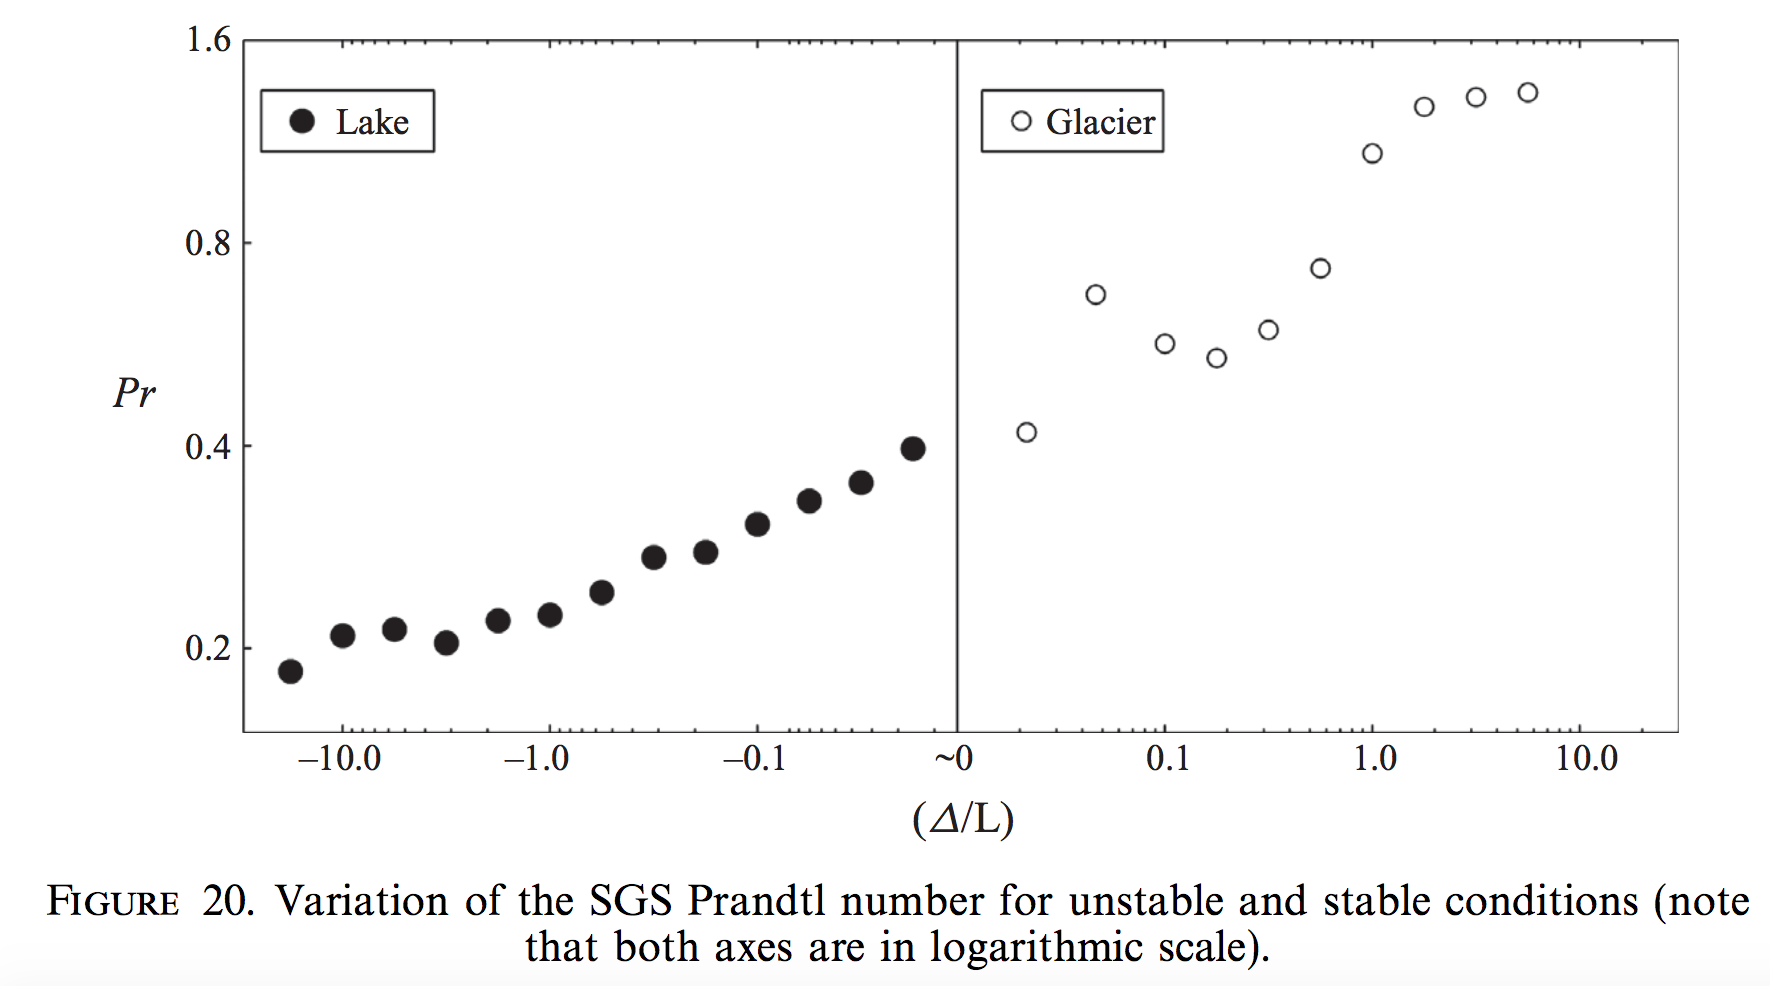
\includegraphics[width=0.7\textwidth]{apriori20}
	\end{figure}
\end{frame}
%------------------------------------------------
\begin{frame}{Geometric Tensor Alignment}
Higgins et al (2003)    
	\begin{columns}
    \begin{column}{.45\textwidth}
    \begin{minipage}[c][.1\textheight][c]{\linewidth}
    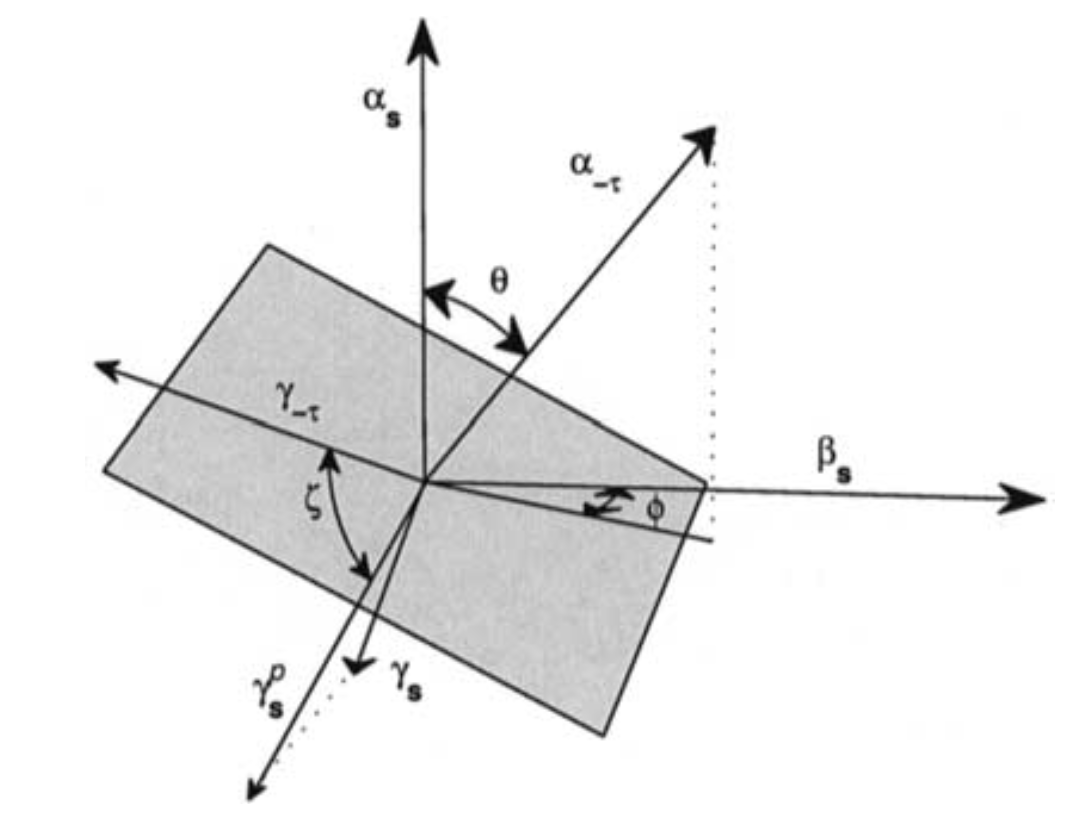
\includegraphics[width=\textwidth]{apriori21}
    ~\\\tiny{Definition of the 3 angles needed to  characterize the alignment of 2 tensors ($\tau_{ij}$ and $S_{ij}$}
      \end{minipage}
    \end{column}
    \begin{column}{.55\textwidth}
    \vspace{-10pt}
      \begin{figure}
      ~\\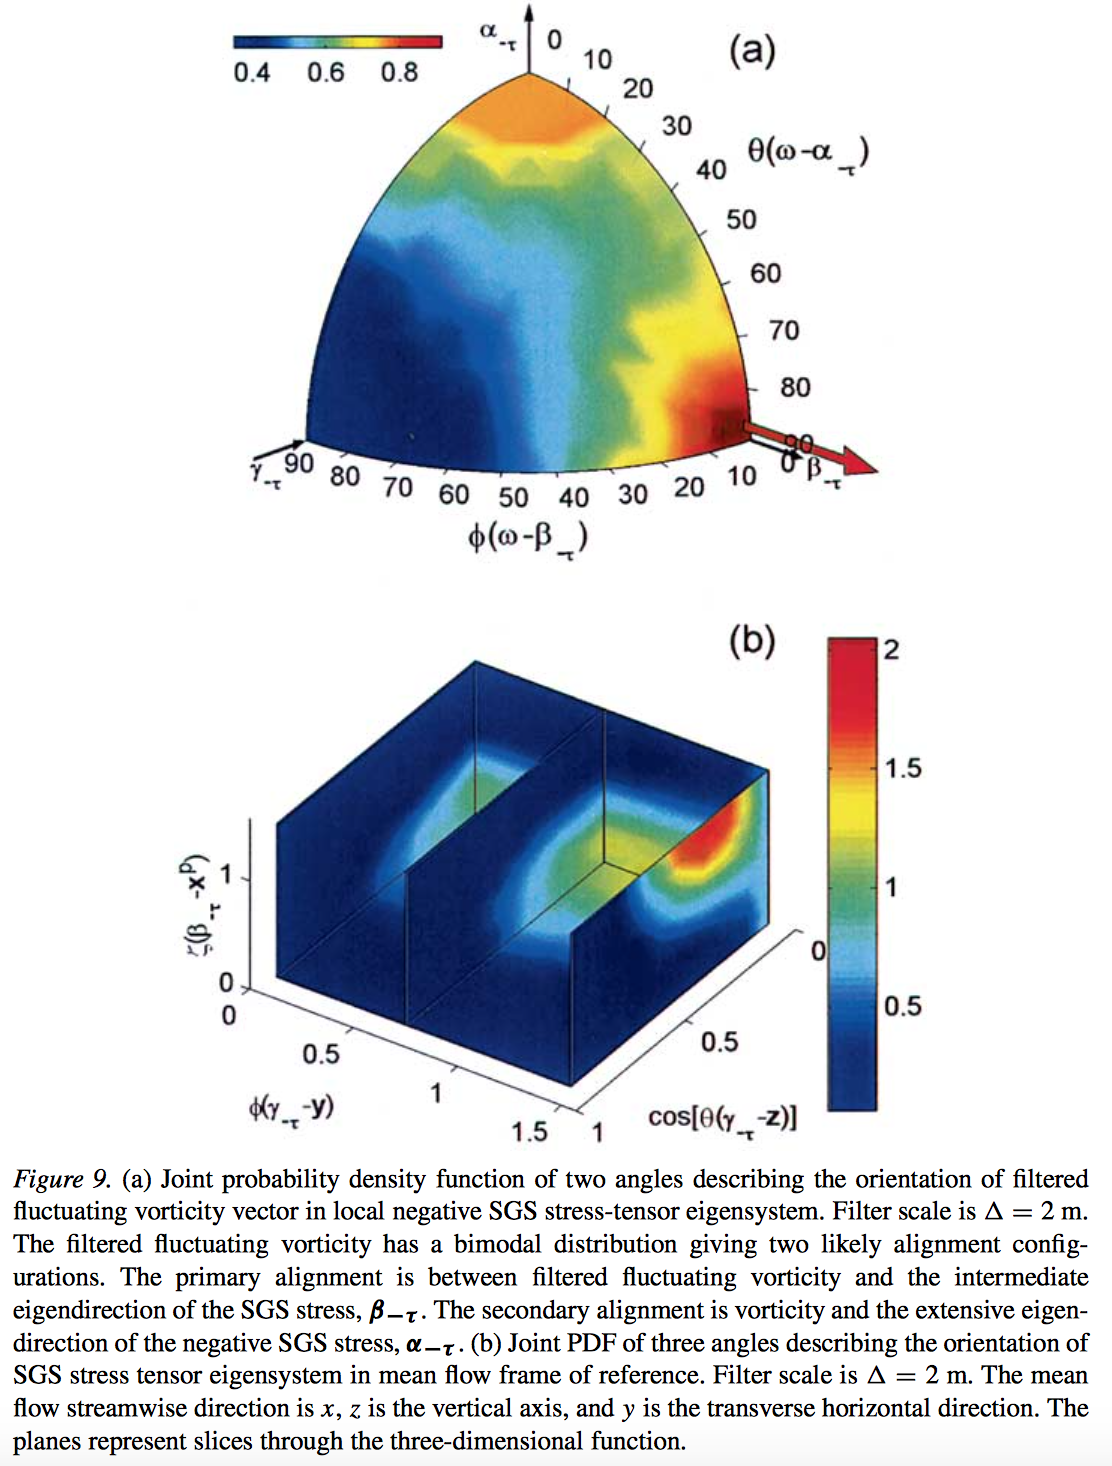
\includegraphics[width=0.90\textwidth]{apriori22}
      \end{figure}
    \end{column}
  \end{columns}
\end{frame}

%------------------------------------------------
\begin{frame}{Geometric Tensor Alignment}
SGS and coherent structures in the Utah desert (Carper and Port\'{e}-Agel 2004)   
	\begin{columns}
    \begin{column}{.45\textwidth}
    \begin{minipage}[c][.1\textheight][c]{\linewidth}
    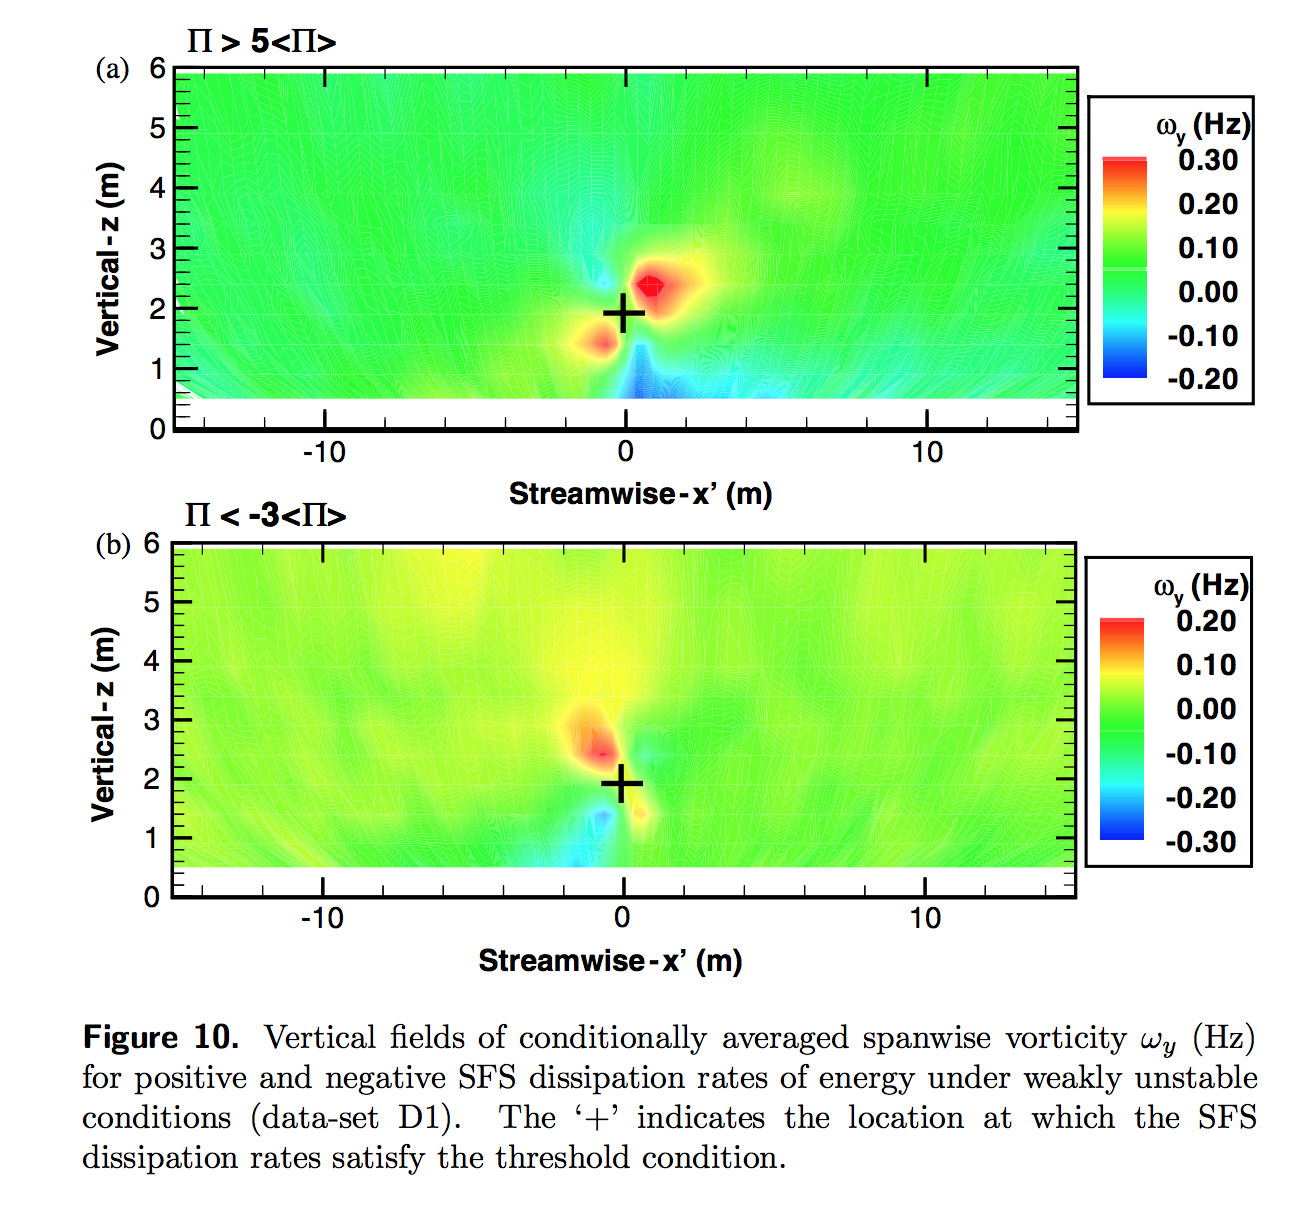
\includegraphics[width=\textwidth]{apriori23}
      \end{minipage}
    \end{column}
    \begin{column}{.55\textwidth}
    \vspace{-10pt}
      \begin{figure}
      ~\\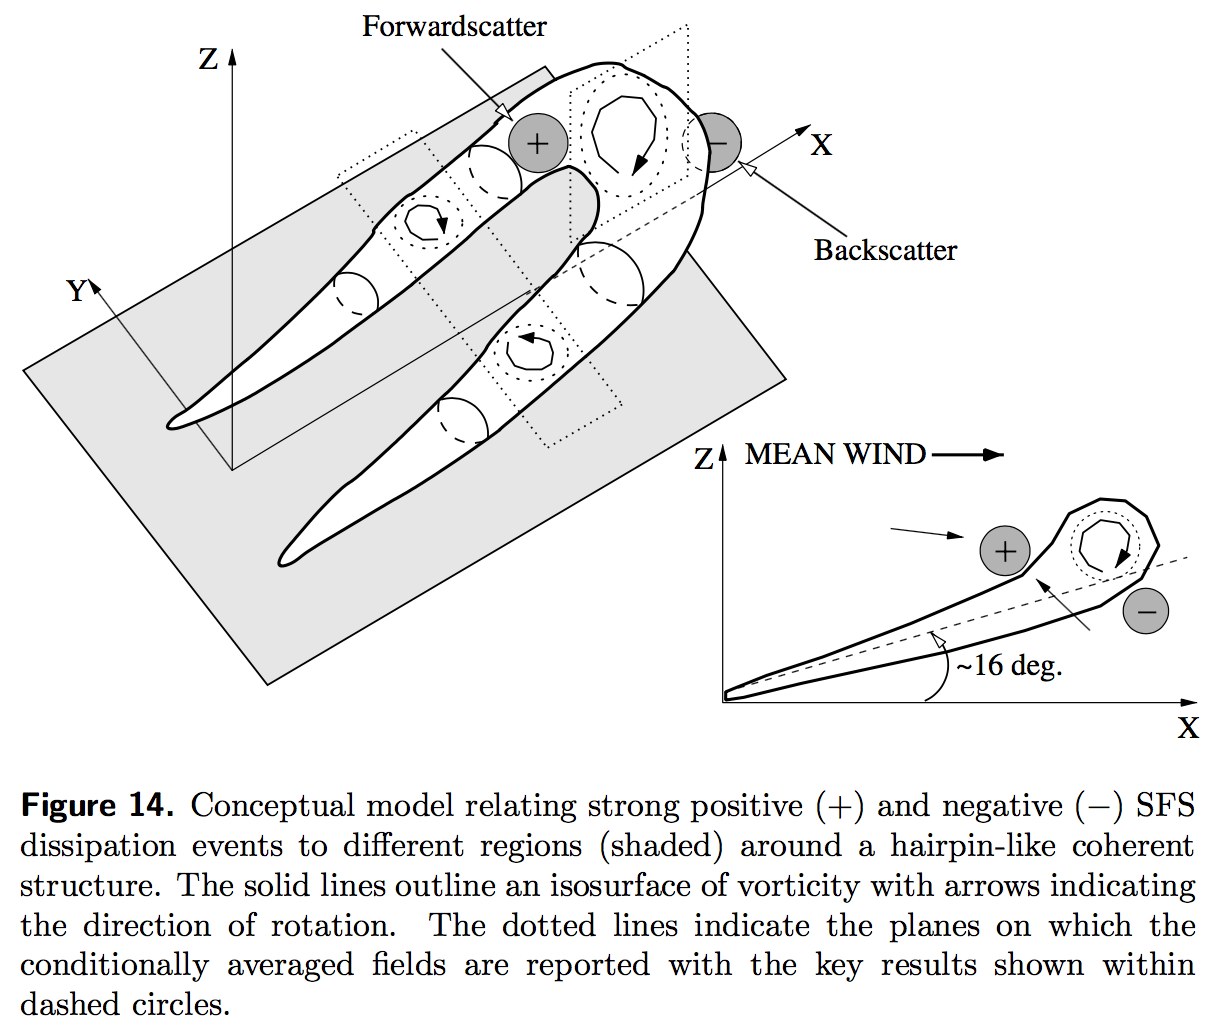
\includegraphics[width=0.90\textwidth]{apriori25}
      \end{figure}
    \end{column}
  \end{columns}
\end{frame}



%------------------------------------------------


\end{document}

